% !TEX TS-program = pdflatex
% !TEX encoding = UTF-8 Unicode

\documentclass[11pt]{article}                                                   % use larger type; default would be 10pt
\usepackage[utf8]{inputenc}                                                     % set input encoding (not needed with XeLaTeX)

%%% PAGE DIMENSIONS ------------------------------------------------------------
\usepackage[top=0.8in, left=1in, right=1in, bottom=0.8in]{geometry}             % to change the page dimensions
\geometry{a4paper}                                                              % or letterpaper (US) or a5paper or....
\usepackage[parfill]{parskip}                                                   % Activate to begin paragraphs with an empty line rather than an indent

%%% HEADERS & FOOTERS ----------------------------------------------------------
\usepackage{fancyhdr}                                                           % This should be set AFTER setting up the page geometry
\pagestyle{fancy}                                                               % options: empty , plain , fancy
\renewcommand{\headrulewidth}{0pt}                                              % customise the layout...
\lhead{}\chead{}\rhead{}
\lfoot{}\cfoot{page \thepage}\rfoot{}

%%% SECTION TITLE APPEARANCE ---------------------------------------------------
\usepackage{sectsty}
\allsectionsfont{\sffamily\mdseries\upshape}                                    % (See the fntguide.pdf for font help)

%%% PACKAGES -------------------------------------------------------------------
\usepackage[font=small,labelfont=bf,textfont=it]{caption}                       % stylize captions
\usepackage{graphicx}                                                           % support the \includegraphics command and options
\usepackage{booktabs}                                                           % for much better looking tables
\usepackage{array}                                                              % for better arrays (eg matrices) in maths
\usepackage{paralist}                                                           % very flexible & customisable lists (eg. enumerate/itemize, etc.)
\usepackage{verbatim}                                                           % adds environment for commenting out blocks of text & for better verbatim
\usepackage{subfig}                                                             % make it possible to include more than one captioned figure/table in a single float
\usepackage{mathtools}                                                          % for math environments like align
\usepackage{amssymb}                                                            % for symbols like \therefore
\usepackage{verbatim}                                                           % for including text as appears, verbatim
\usepackage{listings}                                                           % for including external files as text, eg code
\usepackage{color}                                                              % for coloring of files and images
\usepackage{overpic}                                                            % for adding annotations to pictures
\usepackage{enumitem}

%%% EQUATIONS ------------------------------------------------------------------
\numberwithin{equation}{section}                                                % Number equations by section (change for different levels)

%% BIBIOGRAPHY ------------------------------------------------------------------
\usepackage{cite}
\bibliographystyle{unsrt}

%%% ToC (table of contents) APPEARANCE -----------------------------------------
%\usepackage[nottoc,notlof,notlot]{tocbibind}                                   % Put the bibliography in the ToC
%\usepackage[titles,subfigure]{tocloft}                                         % Alter the style of the Table of Contents
%\renewcommand{\cftsecfont}{\rmfamily\mdseries\upshape}
%\renewcommand{\cftsecpagefont}{\rmfamily\mdseries\upshape}                     % No bold!

%%% PDF LINKS AND STYLE --------------------------------------------------------
\usepackage[unicode=true,
    bookmarks=true,bookmarksnumbered=true,bookmarksopen=true,
    bookmarksopenlevel=2, breaklinks=false,pdfborder={0 0 0},backref=false,
    colorlinks=false] {hyperref}                                                % for links in pdf file, no colors
\hypersetup{pdftitle={DOCUMENT NAME},
    pdfauthor={Josh Wainwright}}                                                % set name of document and author here

%%% END Article customizations

%%% Include TIKZ images directly into document ---------------------------------
\usepackage[svgnames]{xcolor}
\usepackage{tikz}
\usetikzlibrary{decorations.markings}
\usetikzlibrary{shapes.geometric}

\newif\iffinal                                                                  % introduce a switch for draft vs. final document
\finaltrue                                                                      % use this to compile the final document
\usepackage{tikz}

\iffinal
    \newcommand{\inputTikZ}[1]{%
        \input{#1}%
    }
\else
    \newcommand{\inputTikZ}[1]{%
        \beginpgfgraphicnamed{#1-external}%
        \input{#1}%
        \endpgfgraphicnamed%
    }
\fi

%%% Include svg images directly in document (requires Inkscape) ----------------
\newcommand{\executeiffilenewer}[3]{%
    \ifnum\pdfstrcmp{\pdffilemoddate{#1}}%
        {\pdffilemoddate{#2}}>0%
        {\immediate\write18{#3}}
    \fi
}
\newcommand{\includesvg}[1]{%
    \executeiffilenewer{#1.svg}{#1.pdf}%
    {inkscape -z -D --file=#1.svg --export-pdf=#1.pdf --export-latex}%
    \input{#1.pdf_tex}%
}

%%% NEW COMMANDS ---------------------------------------------------------------
\renewcommand{\d}{\,\mathrm{d}}                                                 % for integrals
\newcommand{\dx}[2]{\frac{\textrm{d} #1}{\textrm{d} #2}}                        % for derivatives
\newcommand{\dd}[2]{\frac{\textrm{d}^2 #1}{\textrm{d} #2^2}}                    % for double derivatives
\newcommand{\pd}[2]{\frac{\partial #1}{\partial #2}}                            % for partial derivatives
\newcommand{\pdd}[2]{\frac{\partial^2 #1}{\partial #2^2}}                       % for double partial derivatives
\newcommand{\e}[1]{\text{e}^{#1}}                                               % for exponentials
\newcommand{\code}[1]{\texttt{#1}}                                              % for verbatim code view
\newcommand{\inter}[1]{\shortintertext{#1}}                                     % shorter version of intertext
\newcommand{\under}[1]{\underline{#1}}                                          % for vectors etc.

\let\vaccent=\v                                                                 % rename builtin command \v{} to \vaccent{}
\newcommand{\uv}[1]{\ensuremath{\hat{#1}}}                                      % for unit vector
\newcommand{\abs}[1]{\left| #1 \right|}                                         % for absolute value
\newcommand{\avg}[1]{\left< #1 \right>}                                         % for average
\let\underdot=\d                                                                % rename builtin command \d{} to \underdot{}
\newcommand{\ket}[1]{\left| #1 \right>}                                         % for Dirac bras
\newcommand{\bra}[1]{\left< #1 \right|}                                         % for Dirac kets
\newcommand{\braket}[2]{\left< #1 \vphantom{#2} \right|
    \left. #2 \vphantom{#1} \right>}                                            % for Dirac brackets
\newcommand{\matrixel}[3]{\left< #1 \vphantom{#2#3} \right|
    #2 \left| #3 \vphantom{#1#2} \right>}                                       % for Dirac matrix elements
\newcommand{\grad}[1]{\nabla #1}                                                % for gradient
\let\divsymb=\div                                                               % rename builtin command \div to \divsymb
\renewcommand{\div}[1]{\nabla \cdot #1}                                         % for divergence
\newcommand{\curl}[1]{\nabla \times #1}                                         % for curl
\let\baraccent=\=                                                               % rename builtin command \= to \baraccent
\renewcommand{\=}[1]{\stackrel{#1}{=}}                                          % for putting numbers above =


%*******************************************************************************
%******************************** END HEADER ***********************************
%*******************************************************************************

\begin{document}
%!TEX root = Problems1_main.tex

% Remove the author and date fields and the space associated with them
% from the definition of maketitle!
\makeatletter
\renewcommand{\@maketitle}{
\newpage
 \null
 \vskip 2em%
 \begin{center}%
  {\Large \@title \par}%
 \end{center}%
 \par} \makeatother

\begin{center}
\Huge University Physcis Problems 1\\[1em]
\large 23rd January 2013
\end{center}

\section{Rolling}
Two balls of identical mass and shape with coefficient of friction $\mu=0$, are set rolling at the same initial velocity from point A. Ignoring air resistance, which reaches the end of the track, point B, first and why?
\begin{figure}[ht]
  \centering
  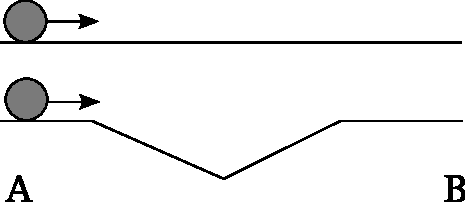
\includegraphics[width=0.4\textwidth]{rolling_balls.pdf}
\end{figure}

\section{Running}
Runners race from point A to point B. The first section is smooth tarmac where there is good grip, the second is soft sand. Which of the five possible paths, a to e, is the fastest and why? Explain your answer.
\begin{figure}[ht]
  \centering
  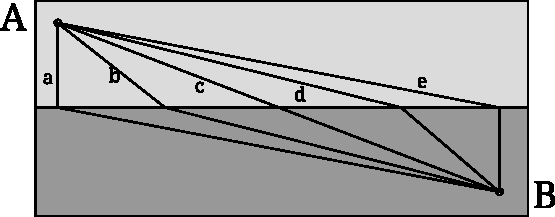
\includegraphics[width=0.6\textwidth]{runners.pdf}
\end{figure}

Which area of physics is the applicable to? How would you solve this numerically?

\section{Dropping}
A slinky is suspended at the top and hangs under its own weight. The top is released. Does the bottom initially:
\begin{enumerate}[label=\alph*)]
	\item move up,
	\item move down,
	\item stay still?
\end{enumerate}

\section{Molecules in the Atmosphere}
Calculate the number of molecules in each of your breaths that was inhaled by Julius Ceasar in his final breath. What assumptions have you made? Use the radius of the earth to be roughly 6\,300\,km.

\section{Floating}
Four vessels each contain a block of floating ice in water. In the first vessel, the ice is solid; in the second, the ice has a large air buble trapped inside; the third has a region of water trapped and the fourth contains a large iron nail.

What happens to the level of the water in each vessel when all the water has melted?
\begin{enumerate}[label=\alph*)]
	\item move up,
	\item move down,
	\item no change?
\end{enumerate}
\begin{figure}[ht]
  \centering
  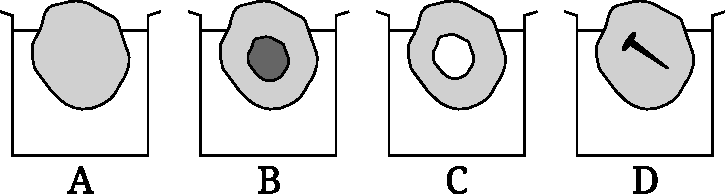
\includegraphics[width=0.8\textwidth]{vessels.pdf}
\end{figure}

\newpage
%!TEX root = Problems1_main.tex

% Remove the author and date fields and the space associated with them
% from the definition of maketitle!
\makeatletter
\renewcommand{\@maketitle}{
\newpage
 \null
 \vskip 2em%
 \begin{center}%
  {\Large \@title \par}%
 \end{center}%
 \par} \makeatother

\begin{center}
\Huge University Physcis Answers 1\\[1em]
\large 23rd January 2013
\end{center}
\setcounter{section}{0}

\section{Rolling}
The first ball reaches B first.

The total displacement is the same in each case, but it is clear that the second ball will travel a greater distance. We must consider the velocity changes. For the flat sections in both cases, the velocity is the same since there is not friction so no way to loose energy. The downill and uphill sections however must change the velocity. 

Looking only at the second case, if we examine the average velocity, we have two sections at the initial velocity, one secion of positive acceleration and one section of negative acceleration. Since, over the range of the dip, the ball must begin and end at the same velocity, these must cancel out. Thus, the total average velocity of the second path is the same as the velocity of the first.

Finally we look at the time taken. The time to cover a distance s is
\begin{align*}
	t = \frac{s}{v}
\end{align*}
Since both paths have the same average velocity, but the second travels further, this must take longer and so the first ball reaches B first.

\section{Running}
d is the fastest route.

This is a problem of minimising the time to travel a given distance. We must take into account the fact that the runner will be able to travel faster on the tarmac than the sand, but that the longer they spend on the tarmac, the further they must travel. A compromise, then, must be made.

c (the shortest overall distance), means the runner spends too long in the sand and so is slowed down too much, however, e (the longest time on the tarmac) means the runner travels to far overall. d then is the best compromise.

This is applicable to light travelling through mediums of different density. It is the same reason that light bends when moving from air to water, or the other way round, making a straw appear to bend. The tarmac is the air in this case, where light travels faster, it then slows down at the boundary with the water, the sand.

The mathematical basis for calculating the exact route taken by the light, or runner, is called Fermat's Principle of Least Time and involves integrating the time taken given the velocity in each medium. This would be covered in first year optics.

\section{Dropping}
The bottom of the slinky will stay still. There are several different explations for this effect. 

\section{Molecules in the Atmosphere}
Assume the following:
\begin{itemize}
	\item The volume of an average breath is 0.5\,litres (actual value 0.3 to 2.0\,litres depending on physical activity, gender etc.)
	\item The atmosphere is roughly 10\,km high (actual value is considerably larger but majority of mass contained within 10-15\,km)
	\item The density of the atmosphere is 1.2\,$\text{kg\,m}^{-3}$ and composed entirely of nitrogen (actual value at sea level but then decreases steadily to zero, and nitrogen is 78\%)
	\item Julius Caesar lived to 50\,years (actually 55)
\end{itemize}
First we need to work out the number of molecules in the whole atmosphere, so we need the volume of the atmosphere. This is approximated as the difference between the volume of the sphere of the earth plus the atmosphere and the sphere of just the earth.
\begin{align*}
	V &= \frac{4}{3}\pi r^3 \\
	V_{atmos} &= \frac{4}{3}\pi \times (6\,300\times10^3 + 10\times10^3) - \frac{4}{3}\pi \times (6\,300\times10^3) \\
	V_{atmos} &= 5\times10^{18}\,\text{m}^3
\end{align*}
This means the mass of the atmosphere is easy to calculate,
\begin{align*}
	M_{atmos} &= \text{density} \times \text{volume} \\
	M_{atmos} &= 1.2 \times 5\times10^{18} \\
	&= 6\times10^{18}\,\text{kg} 
\end{align*}
The average atomic mass of nitrogen is 14, so
\begin{align*}
	14\,\text{g} &= 1\,\text{mol} \\
	14\times10^{-3}\,kg &= N_A\, \text{molecules} \\
	\Rightarrow 1\,\text{kg} &= \frac{N_A}{14\times10^{-3}}\, \text{molecules} \\
	&= 4\times10^{25}\, \text{molecules per kilogram} \\
	\Rightarrow N_{atmos} &= (4\times10^{25}) \times (6\times10^{18}) = 2.5\times10^{44}\, \text{molecules}
\end{align*}
For the number of molecules in each breath, we know that 1\,litre is $10^{-3}$\,m$^3$, so the number of molecules in each breath is $N_{breath}$. 
\begin{align*}
	M_{breath} &= 0.5\times 10^{-3}\times 1.2 = 6\times 10^{-4}\,\text{kg} \\
	\intertext{We know the number of molecules of nitrogen per kilogram, so}
	N_{breath} &= 4\times10^{25}\, \text{molecules per kilogram} \times 6\times 10^{-4}\,\text{kg}\\
	&= 2.4\times10^{22} \,\text{molecules}
\end{align*}
Assuming that, in the intervening time, the molecules from Caesar's last breath are now evenly distributed throughout the atmosphere, when randomly selecting a molecule from the air, there is a small chance that is was one of Caesar's last, given by
\begin{align*}
	P &= \frac{2.4\times10^{22}}{2.5\times10^{44}}
\end{align*}
But since there are such a large number of molecules in each of your breaths, this probability becomes quite high. So for each lungfull of air, there is, on average,
\begin{align*}
	M &= \frac{2.4\times10^{22}}{2.5\times10^{44}} \times 2.4\times10^{22} \\
	&\approx 2
\end{align*}
molecules from Caesar's final breath.


\end{document}
    
